% Quantization at the Entropy Bound — llmopt lab
% Build: tectonic main.tex
% Every numeric claim carries a "% RESULTS L<n>" comment naming the
% docs/RESULTS.md line the number was read from (verified 2026-08-11).
\documentclass[11pt]{article}

\usepackage[letterpaper,margin=1in]{geometry}
\usepackage{amsmath}
\usepackage{amssymb}
\usepackage{booktabs}
\usepackage{graphicx}
\usepackage[T1]{fontenc}
\usepackage[utf8]{inputenc}
\usepackage[hidelinks]{hyperref}

\graphicspath{{figs/}}

\newcommand{\Mstat}{\ensuremath{M}}
\newcommand{\dkl}{\ensuremath{\Delta\mathrm{KL}}}

\title{Quantization at the Entropy Bound:\\
Calibration-Free Packing of At-Capacity Networks}
\author{Artin \\ \small llmopt lab}
\date{}

\begin{document}
\maketitle

\begin{abstract}
Post-training quantization methods earn their complexity on some models and
waste it on others, and current practice offers no way to tell which regime a
model is in without running the quantizers. We give a zero-inference criterion.
A network is \emph{at capacity} when its weight code stream, on a per-row
$\sigma/2$ grid, carries entropy equal to the Gaussian capacity of that grid;
small math-task transformers trained to convergence sit within 1\% of this bound
% RESULTS L10406 (C0+C1), L11238 (n=3 replication)
at $n{=}3$ births on two architectures. At capacity there is little structure
left for calibration to exploit: at matched 5 bits, GPTQ with a real Hessian,
AWQ with real activation profiles, and HQQ all land within one gate sigma of a
closed-form $\sigma$ allocation. % RESULTS L10460
Off capacity, the premium those methods earn is monotone in a disk statistic
$M = \text{span\_bits} - \text{code\_entropy}$ that costs nothing to compute:
measured premiums run from $\sim 1\times$ at $M\,0.96$--$1.61$ (our born
crystals) % RESULTS L10812
through $16.3\times$ at $M\,2.85$ (MoE experts) and $22\times$ at $M\,3.11$
(attention) % RESULTS L10890, L10898
to $34\times$ at $M\,3.62$ (one web-dense LLM). % RESULTS L10908
The meter has been read on five production model families
(OLMoE, Qwen3-30B, DeepSeek-V3, Kimi-K2, Kimi-K3); only one web-dense premium
is actually measured, and the web-dense band spans $M\,3.62$--$3.85$.
% RESULTS L10817-10818
Around the criterion we ship: a closed-form packing artifact whose disk format
is its runtime format (a bit-packed 5-bit Metal GEMV kernel, $2.39\times$ over
fp16 at the best of five benchmarked shapes on synthetic Gaussian weights);
% RESULTS L10593, L10600
a lossless rANS stage reaching $3.67\times$ over bf16 on a 30B MoE with zero
calibration on a laptop; % RESULTS L11303
and a fixed-point decode path whose logit traces are bit-identical across GPU
vendors and laboratories % RESULTS L11364, L11472
--- including on a frontier model's own shipped MXFP4 expert, consumed natively
with zero requantization. % RESULTS L11456, L11518
Every experiment was pre-registered; exploratory reads are labelled as such,
and the falsified predictions are reported alongside the confirmed ones.
\end{abstract}

\section{Introduction}

The quantization literature is a contest of increasingly sophisticated
calibrated methods, each demonstrated on web-trained LLMs, each earning real
margins there. This paper starts from an observation those demonstrations skip:
on some networks, all of that machinery ties a two-line closed-form baseline to
within the resolution of our gate.

The networks where calibration ties are not toys chosen to make the point. They
are transformers trained to convergence on a verified task distribution ---
models we gate-score exactly, so parity claims are measured in solved problems,
not proxy perplexity. On these models we measure (Sec.~\ref{sec:bound}) that the
weight entropy at a fixed quantization step equals the capacity of a Gaussian
source at matched variance to within 1\%. % RESULTS L10406
Nothing in the weights prefers any code over any other; there is little for a
Hessian or an activation profile to find. We call such networks
\emph{at capacity}.

Web-trained LLMs are not at capacity, and the distance from capacity turns out
to be measurable from the weight file alone. Our meter
$M = \text{span\_bits} - \text{code\_entropy}$ prices exactly one thing: what a
fixed-width uniform grid pays to reach the worst outlier in each row.
% RESULTS L10786
Across every group we metered --- born crystals, MoE experts from five
production families, attention blocks, dense web LLMs --- the premium that
calibrated methods earn over the closed form rises with $M$
(Sec.~\ref{sec:meter}). The practical consequence is a decision rule you can run
before loading the model onto an accelerator: below $M \sim 2$, use the closed
form and keep the calibration budget; above it, per-row max-anchored grids and
their calibrated refinements earn their cost. % RESULTS L10916

Three artifacts fall out of taking the entropy bound seriously
(Secs.~\ref{sec:artifact}--\ref{sec:determinism}): a packed format at
$\sim$5 bits/weight whose gate score holds within sigma on our headline class at
$n{=}3$; an entropy-coded container within a rounding error of the measured code
entropy, lossless, at 30B scale on a laptop; and --- because integer codes admit
exact arithmetic --- a decode path that produces bit-identical logit traces on
Apple and NVIDIA silicon, replicated cross-laboratory, and demonstrated on a
frontier MoE's own shipped 4-bit expert format.

Sections~\ref{sec:geometry}--\ref{sec:capmeter} add three measurements that
constrain what the entropy account can and cannot see: bits are blind to the
\emph{geometry} of the grid, the \emph{symmetry} axis carries a separate and
priceable toll, and the meter behaves as a predictive instrument with named
misses. Section~\ref{sec:limits} is the honest-limits section --- where the
method fails, by how much, and at what $n$.

We report our falsified predictions with the same prominence as the confirmed
ones. Several of them sharpened the criterion into its final form; one closes an
entire class of post-hoc MoE compression and redirects the effort to the systems
layer (Sec.~\ref{sec:routing}).

\begin{figure}[t]
\centering
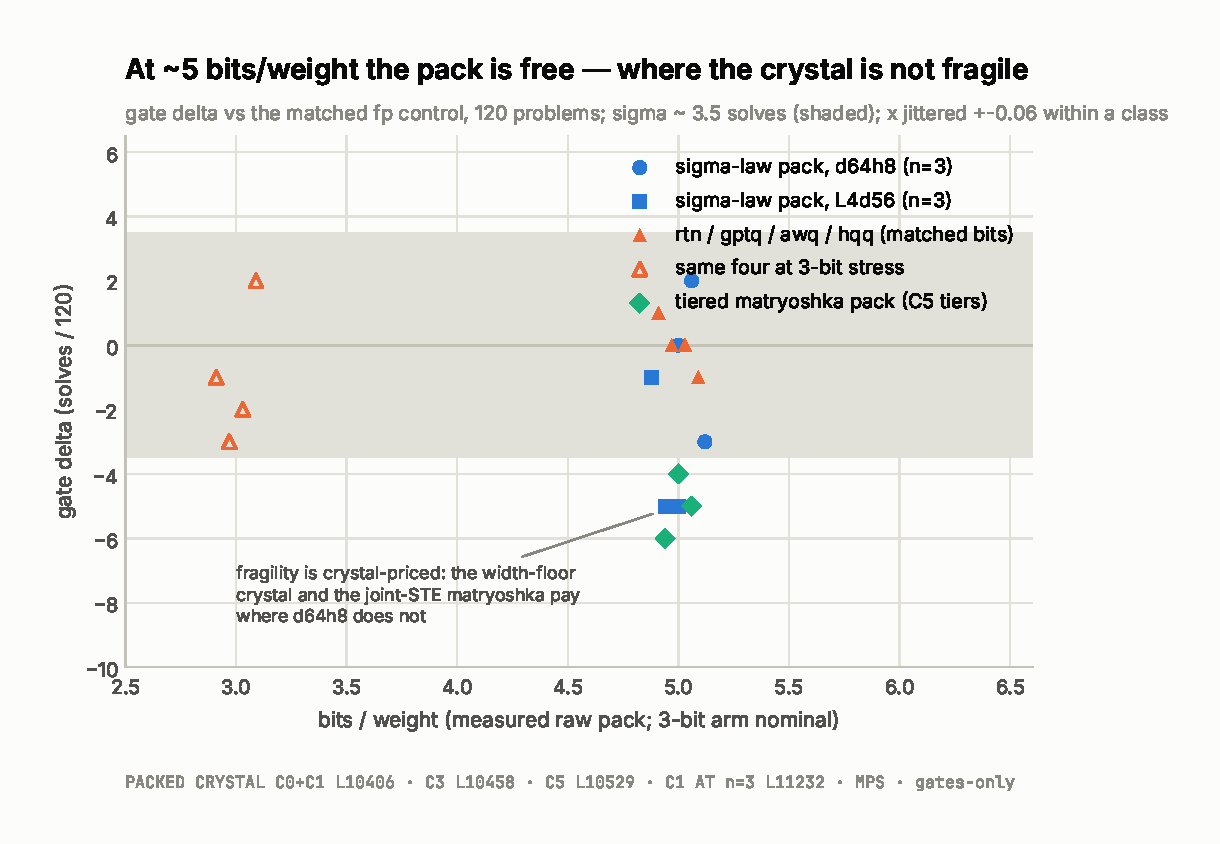
\includegraphics[width=0.86\linewidth]{packing_curve.pdf}
\caption{The packing curve across the C-series cells (C0/C1/C3/C5). The claim:
on at-capacity crystals the closed-form $\sigma$ pack sits at the entropy bound
and calibrated methods do not separate from it at matched bits.
% RESULTS L10406, L10460
Fence: MPS, $n{=}1$ per quantizer arm with C1 controls reused; the parity claim
itself is $n{=}3$ and scoped to the d64h8 class. % RESULTS L10483, L11236
}
\label{fig:packing}
\end{figure}

\section{The entropy bound, measured}
\label{sec:bound}

Fix a weight tensor $W$ with per-row standard deviation $\sigma_r$. Quantize row
$r$ on a uniform grid of step $\sigma_r/2$ and read the resulting integer codes
as a symbol stream. Two numbers describe that stream: its empirical entropy $H$,
and the capacity of a Gaussian source quantized on the same grid,
$H^* = \tfrac{1}{2}\log_2(2\pi e) - \log_2(\text{step}/\sigma)$. If the weights
were drawn i.i.d.\ Gaussian, $H$ would equal $H^*$; any learned structure ---
correlations, heavy tails, clustering --- shows up as $H < H^*$ (compressible
structure) or as grid overhead (outliers stretching the span).

The choice of $\sigma/2$ is set by a separately measured precision knee, not by
the entropy argument. Across three crystals and two widths the knee sits where
the grid step is $0.5$--$1.0\,\sigma$: at $d{=}56$ ($\sigma\!\approx\!0.13$),
$Q{=}16$ is free (grid $0.48\,\sigma$) and $Q{=}8$ bites ($0.96\,\sigma$); at
$d{=}256$ ($\sigma\!\approx\!0.06$), $Q{=}64$ is free ($0.25\,\sigma$) and
$Q{=}16$ bites ($1.0\,\sigma$). % RESULTS L9809-9812
The knee constant was later hardened to $n{=}3$ paired births: $Q{=}64$ within
$\pm 3$ of comparator 3/3 ($0/-1/0$) and $Q{=}16$ at $-7$ or worse 3/3
($-12/-13/-9$), at near-identical sigmas $0.0367$--$0.0369$.
% RESULTS L22662-22670
So $\sigma/2$ is a step comfortably inside the free zone, not ``the coarsest
step that keeps parity.''

Measured on our born crystals (d64 8-head and layers-4 d56 math-task
transformers), $H$ sits within 1\% of $H^*$: code entropy $3.10$--$3.13$ against
capacity $\approx 3.13$ on all four birth/architecture cells at $n{=}3$.
% RESULTS L11237-11239
This is the paper's anchor measurement: these networks are \emph{at capacity}
--- maximum-entropy on their own grid, with little left for a smarter code to
find.

The at-capacity state has a sharp operational consequence, verified directly in
Sec.~\ref{sec:artifact}: every calibrated quantizer we tested lands inside the
gate's resolution of the closed form. And it has a converse: any model whose
code stream falls short of capacity, or whose span outruns its entropy, is
\emph{not} at capacity, and the shortfall is exploitable --- by exactly the
methods the literature already built. The rest of the paper measures that gap and
the toolchain that lives on its floor.

\section{The meter: regime detection from disk}
\label{sec:meter}

$M = \text{span\_bits} - \text{code\_entropy}$, computed at per-row $\sigma/2$,
no forward passes. Span\_bits is what the fixed-width grid must pay per weight;
code\_entropy is what the weights actually carry. Their difference prices the
worst-case outlier against the typical weight --- mechanically the same thing a
calibrated outlier-aware method gets paid for handling well. % RESULTS L10786-10790

\begin{table}[t]
\centering
\caption{The dial. $M$ at per-row $\sigma/2$, param-weighted, alongside the
measured calibration premium ($\sigma$-allocation \dkl{} divided by HQQ's
\dkl{}, same device, matched bits). Premiums are measured only where a premium
column is given; the rest are meter-only rows.}
\label{tab:dial}
\begin{tabular}{lrrl}
\toprule
group & $M$ & kurtosis & measured premium \\
\midrule
crystal cplx\_none            & 0.96 & 2.26 & --- \\ % RESULTS L10812
crystal d64h8                 & 1.61 & 3.70 & $\sim 1\times$ (ties at gate) \\ % RESULTS L10813, L10460
crystal L4d56                 & 1.61 & 3.56 & --- \\ % RESULTS L10814
house NNUE                    & 0.82 & ---  & --- \\ % RESULTS L10917 (in-passing C7 assertion)
Kimi-K3 experts ($\sim$33M)   & 1.94--2.15 & 3.12 & --- \\ % RESULTS L11443
Kimi-K2 experts ($\sim$40M)   & 2.01 & 3.02--3.04 & --- \\ % RESULTS L11059, L11189
DeepSeek-V3 experts ($\sim$45M) & 2.33 & 3.07 & --- (predicted 5--10$\times$, unmeasured) \\ % RESULTS L10815, L10918
OLMoE experts ($\sim$6M)      & 2.85 & 3.50 & $16.3\times$ \\ % RESULTS L10890, L10898
Qwen3-30B experts ($\sim$5M)  & 2.93 (median) & --- & --- \\ % RESULTS L11049, L11058
OLMoE attention               & 3.11 & 7.55 & $22\times$ \\ % RESULTS L10890, L10900
Qwen2.5-0.5B dense            & 3.62 & 5.29 & $34\times$ \\ % RESULTS L10817, L10908
SmolLM2-1.7B dense            & 3.85 & 6.54 & --- \\ % RESULTS L10818
\bottomrule
\end{tabular}
\end{table}

Table~\ref{tab:dial} is the instrument. Two caveats travel with it and we state
them here rather than in a footnote. First, the ``NNUE 0.82'' row is an
in-passing assertion made in the C7 verdict text, not a cell with its own
receipt; we keep it only with that label. % RESULTS L10917
Second, exactly \emph{one} web-dense premium is measured
(Qwen2.5-0.5B at $M\,3.62 \to 34\times$); SmolLM2-1.7B at $M\,3.85$ was metered
but never given a $\sigma$-vs-HQQ premium arm, so the web-dense band is
$3.62$--$3.85$ in $M$ with a single premium anchor.
% RESULTS L10817-10818, L10908

Two falsifications built this instrument, and we report them as such. First,
``strong transport'' --- the claim that $\sigma$ allocation would hold on any
expert-shaped tensor --- failed on OLMoE experts ($16.3\times$ premium to HQQ at
matched 6 bits); the meter had flagged the miss before the arms ran, in an
amendment written at kill time, which is what promoted it from diagnostic to
dial. % RESULTS L10888-10893, L10901-10911
Second, kurtosis, the obvious moment statistic, is demoted by measurement: the
OLMoE expert group read kurtosis $3.50$ --- nominally Gaussian --- while
carrying $M\,2.85$ worth of grid overhead. % RESULTS L10890, L10922-10924

The dial comes with a second condition, also learned from a falsification:
zero-tax deployment requires an evaluation metric with knee slack. Under outcome
scoring (does the model still solve the task), our packs are free below
$M \sim 2$; under per-token KL, nothing is free --- on OLMoE experts the dial
policy read \dkl{} $0.0187$/tok against RTN's $0.0097$, i.e.\ $1.9\times$
\emph{worse}. % RESULTS L11136-11138
We argue outcome scoring is the deployment-realistic metric, and we say
explicitly that this is an argument, not a theorem.

\paragraph{Expert size, and where the trend breaks.}
A scaling regularity was proposed on the MoE rows: expert capacity tracks
\emph{per-expert size}, not expert count --- Qwen3-30B ($\sim$5M/expert) at
$M\,2.93$, OLMoE ($\sim$6M) at $2.85$, DeepSeek-V3 ($\sim$45M) at $2.33$,
Kimi-K2 ($\sim$40M) at $2.01$. % RESULTS L11058-11059
We state the tension in the same breath: this ordering is \emph{not} monotone in
size. The 45M-parameter DeepSeek experts read $2.33$ while the smaller 40M
Kimi-K2 experts read $2.01$, and Kimi-K3's $\sim$33M experts read
$1.94$--$2.15$, below both. % RESULTS L10815, L11059, L11443
The K3 row additionally carries a grid-image confound: K3 ships MXFP4, so the
meter reads the shipped 4-bit image, which caps span and biases $M$ low. The
honest statement is a \emph{band} --- large experts sit near $M \approx 2.0$, at
the $\sigma$-law boundary --- not a rank ordering. % RESULTS L11446-11450

Frontier practice is consistent with the band. Kimi-K3 ships 896 experts
\emph{per layer} across 93 layers % RESULTS L11125
in a latent MoE (experts read a 3584-dim latent, so an expert is $\sim$33M
parameters, not the $\sim$66M naive estimate --- a figure we established by
pulling a single expert from the 2.8T release by HTTP byte-range).
% RESULTS L11439-11442
Its shipped 4-bit codes carry $3.643$ bits/param, so MXFP4 leaves roughly 9\%
lossless margin: Moonshot packs within $\sim 0.36$ bits of its own format's
capacity. % RESULTS L11450-11453

\begin{figure}[t]
\centering
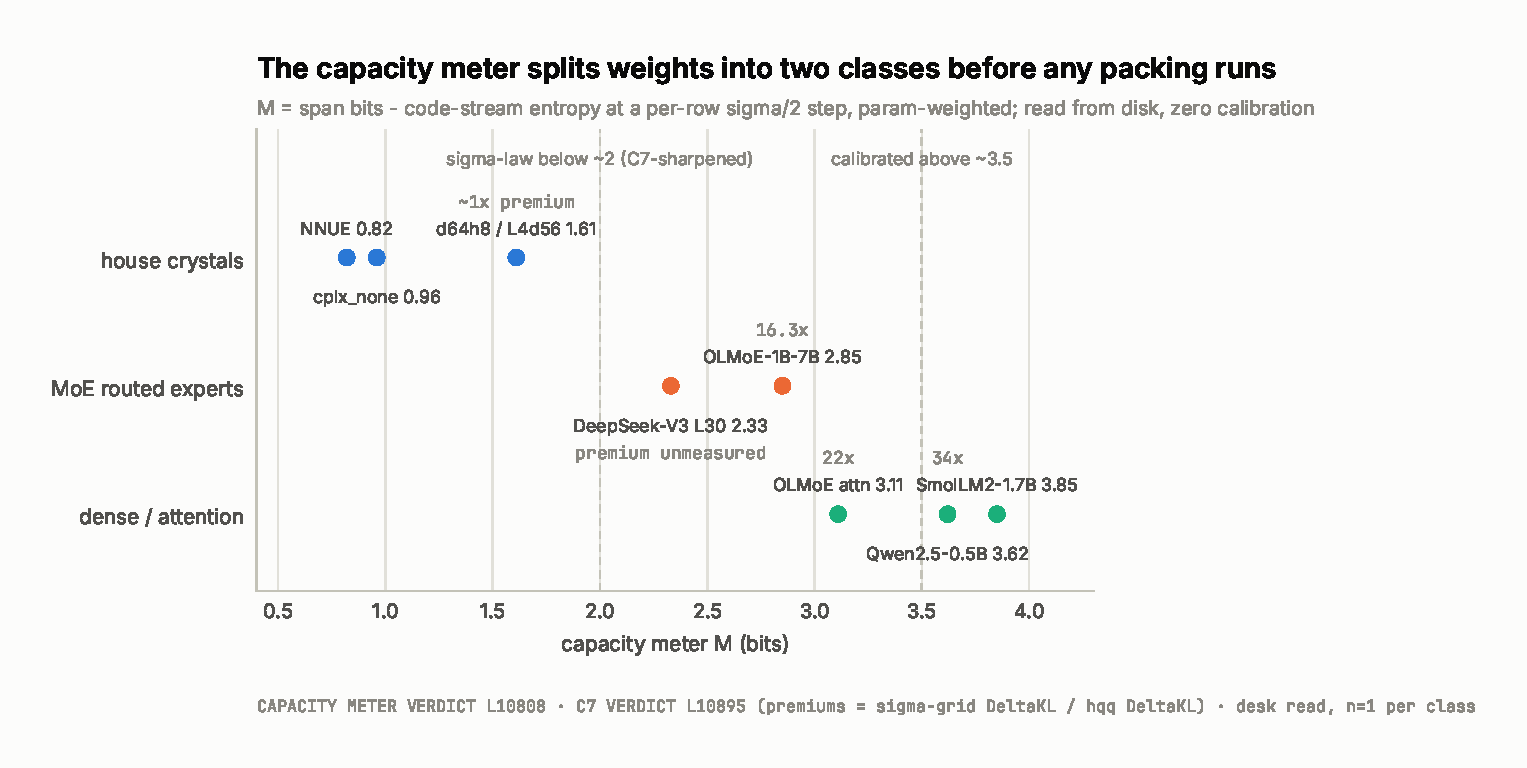
\includegraphics[width=0.86\linewidth]{capacity_meter.pdf}
\caption{The capacity meter as a dial. The claim: the calibration premium rises
with $M$ across the measured groups. % RESULTS L10808-10818, L10895-10916
Fences: premiums are single-model, $n{=}1$ per arm, same-device paired; the
DeepSeek row's $5$--$10\times$ is a \emph{predicted}, unmeasured premium
% RESULTS L10918-10920
and quantized-release rows (K2, K3) read the shipped grid's image, not the fp
master. % RESULTS L11446-11450
}
\label{fig:meter}
\end{figure}

The atlas cell shows the meter at production scale: Qwen3-30B, 30.2B parameters
across 18{,}673 tensors, metered and dial-packed in a 136.6-minute laptop pass
with zero calibration. % RESULTS L11047, L11070
Routers are the incompressible organ ($M\,4.45$, all top-5 function errors are
routers --- keep them fp); expert up\_proj reads median $M\,1.93$, already inside
the $\sigma$-law domain, against gate/down at $2.93$. % RESULTS L11049-11055
The mid-stack dip the atlas found (layers $\sim$8--16 at $M\,1.93$) did
\emph{not} generalize: Kimi-K2 reads flat in depth ($2.09/2.04/2.09$), so the dip
is a recipe or scale artifact, not a law. % RESULTS L11052, L11189-11192

\section{The artifact: packing at the bound}
\label{sec:artifact}

The packing rule is two lines. For each 2-D block tensor $t$ with standard
deviation $\sigma_t$, choose the integer grid $q_t = \lceil 2/\sigma_t \rceil$
--- i.e.\ step $\sigma_t/2$ --- round, and store the codes bit-packed at the
width the span requires ($\sim$5 bits/weight on our models). Embedding, head and
norm tensors stay fp32 in the booked artifact: they are tiny and were never
snapped. % RESULTS L10380-10385
(A separate $\sigma/8$ interface-tensor knob was tried in the fixed-point decode
work and changed nothing; we do not ship it.) % RESULTS L11373
No calibration data, no optimization, no inference.

\paragraph{Parity.}
On the d64h8 class, the pack holds gate parity within sigma at $n{=}3$: seed 1
$58 \to 58$, seed 2 $54 \to 56$ ($+2$), seed 3 $59 \to 56$ ($-3$) --- all three
deltas below the gate sigma of $3.5$. % RESULTS L11234-11237
Seed 1 is exact; the class-level claim is parity within sigma, not exactness. On
the layers-4 d56 depth-floor class the pack pays $-5$ at both new seeds
($50 \to 45$, $52 \to 47$) against seed 1's $-1$; two readings beyond sigma is
not noise. % RESULTS L11239-11241
We therefore scope the zero-tax claim to the d64h8 class and name per-crystal
fragility (Sec.~\ref{sec:limits}) as the axis the entropy argument does not see.
Compression is $6.15$--$6.65\times$ over fp32. % RESULTS L10421-10422

\paragraph{The tie.}
At matched 5 bits on at-capacity weights, GPTQ with its real Hessian (58), AWQ
with real activation profiles (58), HQQ with its per-tensor optimization (57)
and plain RTN (59) all land within sigma of both the fp control (58) and our
pack (58); \dkl{} runs $0.0011$--$0.0018$/tok. % RESULTS L10460-10462
This is an underpowered null at $n{=}1$ per arm, not a demonstration of
equality: the correct reading is that no calibrated method separates from the
closed form at this resolution. A 3-bit stress arm shows where damage lands when
it does come: solve rates stay flat (rtn 57, gptq 55, awq 56, hqq 60 --- the
pre-registered $>\!\sigma$ drop did \emph{not} fire) while validity falls from
57\% to 46--54\% and \dkl{} jumps 20--40$\times$. % RESULTS L10466-10469

\paragraph{Wall-time is calibration time.}
The pack runs in 0.9\,s where HQQ takes 61.7\,s at 0.5B scale ($69\times$), and
16.6\,s where HQQ takes 675.5\,s on 6.4B expert parameters ($41\times$).
% RESULTS L10684, L10914-10915
Two honest qualifications. First, these are \emph{calibration-time} numbers, not
inference-time. Second, and more important: both cells come from C6 and C7,
which are precisely the regimes where our transport claim \emph{failed}. Where
parity actually holds --- the 200k--500k-parameter crystals --- calibration is
sub-second (0.9\,s pass, $<\!0.2$\,s optimize) and the wall-time differentiator
is trivial. % RESULTS L10478-10481
The speed gap is real but it is not evidence for the closed form in the regime
the closed form wins.

\paragraph{The disk format is the runtime format.}
A Metal GEMV kernel consumes the bit-packed 5-bit codes directly --- six signed
codes per uint32, no unpack pass. Across five benchmarked shapes it reads
$1.11\times$ ($224{\times}54$), $1.21\times$ ($256{\times}66$), $1.07\times$
($1536{\times}384$), $1.73\times$ ($8192{\times}2046$) and $2.39\times$
($14336{\times}4098$) over fp16, beating the byte-aligned variant of the same
kernel at the same shape class (1.76$\times$): the denser format wins on
bandwidth. % RESULTS L10592-10596
The $2.39\times$ headline is the best of those five shapes, on synthetic
Gaussian weights at crystal sigma (0.19), $n{=}1$ per shape.
% RESULTS L10600-10601
The honest losses: at micro shapes the kernel is parity-within-noise --- a
$256{\times}64$ cell read $0.91\times$ once and $1.03\times$ on replication, and
micro-shape entries are fenced accordingly. % RESULTS L10850-10852
The one clean ``first attempts lost'' story belongs to a different kernel line:
the int4 dequant-GEMV ladder went $0.47$--$0.70\times$ (v1), $0.75$--$1.00\times$
(v2), $1.11\times$ at $D{=}4096$ (v3). % RESULTS L1193-1195

\paragraph{One negative fences the artifact class.}
On a jointly-trained matryoshka (tiered) crystal, every tier of the nested pack
pays 1--2 sigma. Tiered packing is real ($-15\%$ bytes per solve under escalation
economics) but its zero-tax version requires packing EMA parents, not joint-STE
children. Fragility, again, is orthogonal to entropy ($n{=}1$).

\section{Lossless coding: the bound as bytes}
\label{sec:rans}

If the code stream carries $H$ bits/weight, an entropy coder should store it in
$H$ bits/weight, and the meter already measured $H$ from disk. A range coder
(rANS) over the $\sigma$-law codes achieves that. The pre-registered prediction
was that streams land within 0.5\% of entropy, and it confirmed --- but the
\emph{artifacts} carry table overhead on top: the d64h8 artifact is 233{,}180
bytes ($9.10\times$ over fp32) at $3.179$ bits/wt against a code entropy of
$3.12$, i.e.\ $+1.9\%$; L4d56 reads $8.25\times$; all six seed crystals sit in a
$3.16$--$3.21$ bits/wt band. % RESULTS L11299-11307
Tables add roughly 2\% on the small crystals, counted honestly; there is no
0.1\% claim.

At scale: the packed-plus-coded Qwen3-30B artifact is 16.48\,GB (codes $4.337$
bits/wt $+$ 0.09\,GB scales) against the 60.4\,GB bf16 release --- $3.67\times$
smaller, lossless, produced on a laptop in one pass with zero calibration.
% RESULTS L11302-11304
Losslessness is asserted per stream, with the first 2B Qwen symbols explicitly
roundtrip-verified and coder identity relied on thereafter. % RESULTS L11308-11310
The pipeline composes: rANS is the at-rest container, and decompression yields
the same bit-packed codes the Sec.~\ref{sec:artifact} kernel executes, so the
storage format and the execution format are two states of one object.
Fences: $n{=}1$ per artifact; decode-side rANS throughput is not benched.
% RESULTS L11317-11320

\section{Determinism: exact arithmetic as a deployment property}
\label{sec:determinism}

Integer codes admit exact arithmetic, and exact arithmetic is order-invariant:
an int64 sum gives the same bits under any reduction schedule, which is
precisely what floating-point inference cannot promise across GPUs. We build
this out in three stages, each verified by hash equality, not tolerance.

\paragraph{Stage 1 --- exact GEMMs.}
Weights as integer codes, GEMMs on an exact-fp32 carrier with hi/lo splitting
keeping every partial below $2^{24}$ (the fp32 mantissa bound, asserted at
runtime). The cell books \emph{two hash channels}, not two seeds: hash A (integer
GEMM over all $\sigma$-law code tensors) is bit-identical on MPS and cuda, while
hash B (the fp32 full-forward logits) differs across the same pair; greedy
streams match anyway, per the near-tie doctrine. % RESULTS L10659-10667
A replication pass re-ran hash A on a second \emph{activation} battery seed and
it reproduced identically. % RESULTS L10842-10845

\paragraph{Stage 2 --- full fixed-point decode.}
RMSNorm as int64 sums-of-squares with integer-Newton isqrt; SiLU, softmax-exp and
RoPE as integer tables generated once and shipped as bytes (libm variation across
platforms is exactly the thing being excluded, so tables must travel, never be
regenerated). The complete per-step logit \emph{traces} --- every number, not
just the argmax --- hash identically on MPS and cuda, with max GEMM partial
$2^{21.2}$ against the $2^{24}$ bound. % RESULTS L11364-11367
The capability price, measured honestly: 96.66\% teacher-forced argmax agreement
against the fp parent over 3{,}055 tokens, with disagreements concentrated at
coin-flip margins (median 0.177 vs 7.6 overall); the reference implementation
runs 10--40$\times$ slower than fp, and speed is not the claim.
% RESULTS L11369-11381
An independent laboratory reproduced both digests from the sha-pinned tables
file on first attempt, giving one tables file across cpu, MPS (two machines) and
cuda, in two labs, with no tolerance column. % RESULTS L11471-11480
This cross-lab leg covers the Stage-2 (P3) result only, and the second lab's
contribution was its MPS leg.

\paragraph{Stage 3 --- a frontier model's own format.}
Kimi-K3's routed experts ship as MXFP4: e2m1 integer codes times power-of-two
scales --- already exact. We pulled one expert (17.5\,MB by safetensors
byte-range, out of a 2.8T release), consumed the shipped codes natively with zero
requantization, and measured sha-identical integer-GEMV traces on cpu, MPS and
cuda for all three matrices. % RESULTS L11435-11457
A follow-up cell closed the composition fence: the full expert \emph{forward}
(w1/w3 GEMVs $\to$ power-of-two requant $\to$ shipped SiLU table $\to$ gate$\times$up
$\to$ w2 GEMV) hashes identically on the same three backends.
% RESULTS L11515-11518
Both K3 cells are house-only, on a synthetic 64-vector battery, and are an
\emph{expert forward}, not a full-model decode. % RESULTS L11524
Two experts were metered; one was hash-locked at both GEMV and chain level.
% RESULTS L11443, L11515

\section{Bits are geometry-blind}
\label{sec:geometry}

The entropy account makes a strong implicit claim: what a quantization grid costs
a network depends on the \emph{information} the grid destroys, not on the
coordinate system the grid is drawn in. We tested that directly, four ways, and
it survived all four.

\paragraph{Polar versus Cartesian grids.}
On a complex-FFN crystal (cplx\_none, $d{=}384$, control 63), we swept uniform
$\sigma$-step grids against polar grids that quantize magnitude and angle
separately. The uniform arm obeys the $\sigma$-priced knee as predicted
($0.5\sigma$ free at 63, $2\sigma$ bites to 60). The pre-registered prediction
that polar wins at matched measured bits was falsified: 4.75-bit polar reads 61
against 4.62-bit uniform's 60 --- parity, sub-sigma, not a win.
% RESULTS L10240-10246
The angle-starvation prediction was falsified too: \emph{eight} angle bins are
free at fine magnitude (63 solves at 6.23 bits/weight). % RESULTS L10247-10248
The law that books: the snap knee follows total measured bits/weight regardless
of grid geometry. % RESULTS L10249-10251

\paragraph{Rotating the grid under star-shaped weights.}
The obvious objection is that cplx\_none's weights are isotropic, so no
coordinate frame is special. We re-ran on a ``star'' crystal (cplx\_G5\_dep,
control 66) whose weights are strongly anisotropic. A 45-degree grid rotation
moves every nonzero star weight by $|\delta c| \approx 0.77|c|$ --- massive
distortion --- and cost 1 solve against the aligned grid: polar4 aligned 63,
polar4 rotated-45 62, uniform 63. % RESULTS L10336-10340
The aligned-free/misaligned-craters prediction was falsified. Anisotropic weights
do not imply axis-priced quantization.

\paragraph{No spontaneous rotational structure to align to.}
A complementary read explains why. Measuring anti-commutant mass against an
adjacent-pairing complex structure, every real crystal sits inside the
random-pairing null band at $\approx 0.500$ (wfloor $0.49983$, s2 $0.50022$,
muon $0.50045$, 19m $0.50021$) --- there is no hidden rotational subspace for a
rotated grid to respect. % RESULTS L8482-8486
Projecting the gate matrices onto the commutant gives a strikingly gentle damage
curve: $t{=}0$: 65, $t{=}0.25$: 65, $t{=}0.5$: 64, $t{=}1.0$: 57 --- deleting
50\% of gate mass into the commutant costs 8 solves. % RESULTS L8576-8578
One warm epoch under a ramped commutation penalty heals that back to 64 at
anti-mass $2\times 10^{-4}$. % RESULTS L8615-8616

\paragraph{The alphabet does not have to follow the domain.}
The sharpest version of the geometry question was run on a ZX-calculus diagram
task, where the data itself carries phases: does a rotational (complex) weight
alphabet beat a scalar magnitude alphabet on phase-carrying data? Rotational
read 32/120 against magnitude's 31/120 with a pre-registered bar of $\geq 5$;
alphabet-follows-domain is dead. The same tie holds on the math diet (62 = 62).
% RESULTS L6659-6666

Fences for this section: single-seed cells, MPS (the ZX column excepted, cuda),
and gate/up matrices only.

\section{The symmetry axis and its toll curve}
\label{sec:symmetry}

Bits are one compression currency. \emph{Structure} --- imposing a group symmetry
on the weights so that $k$ parameters share one degree of freedom --- is another,
and it prices differently. We measured a ladder of impositions on the same
trained crystal (comparator 65/120), each by the same recipe: project the gate
matrices onto the commutant of the group, then heal for one warm epoch under a
ramped commutation penalty.

\begin{table}[t]
\centering
\caption{The symmetry ladder. Each rung projects a trained crystal's gate
matrices onto a group's commutant, then heals one epoch. Comparator 65/120,
$n{=}1$ per arm, gates-only, MPS.}
\label{tab:ladder}
\begin{tabular}{llrrrr}
\toprule
rung & group & sharing & projected init & healed gate & anti-mass \\
\midrule
R3 & complex     & $2\times$ & 57 & 64 & $2\times10^{-4}$ \\ % RESULTS L8577, L8616
S1 & quaternion  & $4\times$ & 22 & 61 & $7\times10^{-4}$ \\ % RESULTS L8688-8690
S4 & $Z_2$       & $2\times$ & 49 & 64 & $2\times10^{-4}$ \\ % RESULTS L8742
S3 & $C_8$ (block-circulant) & $8\times$ & 2 & 59 & $2.8\times10^{-3}$ \\ % RESULTS L8743
\bottomrule
\end{tabular}
\end{table}

The toll curve reads $2\times$: $-1$ solve, $4\times$: $-4$, $8\times$: $-6$
(Table~\ref{tab:ladder}). The remarkable cell is S3: dense gate matrices of a
trained crystal retrofit into block-circulant (convolution) structure at
$8\times$ parameter sharing, healing from a projected init of 2/120 to 59/120.
% RESULTS L8744-8747
The no-spontaneous-structure null holds at all three groups tested (complex,
quaternion, $Z_2$/$C_8$) --- these symmetries must be imposed, never found.
% RESULTS L8735-8739

\paragraph{Exactness is available, at a width price.}
Doubling the crystal's width ($d\,256 \to 512$, $W \oplus W$ everywhere, head
$[W/2 | W/2]$, heads $4 \to 8$ at fixed head\_dim) produces an
\emph{exactly} complex-linear model: all eight doubled gates assert anti-mass
$< 10^{-12}$, and the gate reads exactly 65/120 --- the comparator, with no
floating-point tie flipped. % RESULTS L8790-8792
So both endpoints of the trade are measured: exact at $2\times$ width (cost:
$4\times$ params) versus healed at $1\times$ width (cost: $\sim1$ solve,
params/2). Compression and exactness pull opposite ways on this axis.

\paragraph{The $4\times$ toll, hardened.}
The quaternionic rung was the one worth $n{=}3$. Against comparator 65, three
data-order seeds read $59$ ($-6$), $59$ ($-6$) and $60$ ($-5$), pooled $-17$,
3/3 negative, every heal at anti-mass $\leq 7\times10^{-4}$. % RESULTS L23178-23182
The $4\times$ toll is therefore best quoted as \textbf{5--6 solves} at $n{=}3$,
not the single-seed $-4$. (The replication variable had to be found: the torch
seed measured inert in this driver, so the hardening seeds redirect the driver's
hardcoded data-order shuffle.) % RESULTS L23170-23175

\paragraph{The axes are not orthogonal --- except when they are.}
Two cells bracket the interaction. On the 19M crystal, quantization and sharing
compete for one slack budget: at $Q{=}16$ the dense substrate pays $-12$ (65 to
53) while the circulant-$8\times$ substrate pays $-25$ (59 to 34), a
delta-of-deltas of $-13$ against a gate sigma of 3; at $Q{=}8$ both are
destroyed. % RESULTS L8963-8971
But a later cell on the star lineage found the opposite for a different pairing
of axes: $4\times$ quaternionic sharing changed the ternary-sensitivity profile
by nothing --- retention fractions of each arm's \emph{own} base are equal class
by class (emb 62\% vs 58\%, head 102\% vs 100\%, attn 0\% vs 0\%, ffn 26\% vs
26\%). % RESULTS L26038-26044
The reconcilable reading is that the compression corner measures a shared slack
\emph{pool} at a fixed harsh grid, while the ternary profile measures the
\emph{shape} of sensitivity across locations; sharing consumes the former and
leaves the latter untouched.

A third asymmetry is worth naming because it rules out a tempting story: $Z_2$
and complex both share parameters $2\times$, but their projected inits differ
sharply (49 vs 57) --- equal mass removed, unequal damage. Structure, not mass,
is what the toll prices. % RESULTS L8577, L8742

\begin{figure}[t]
\centering
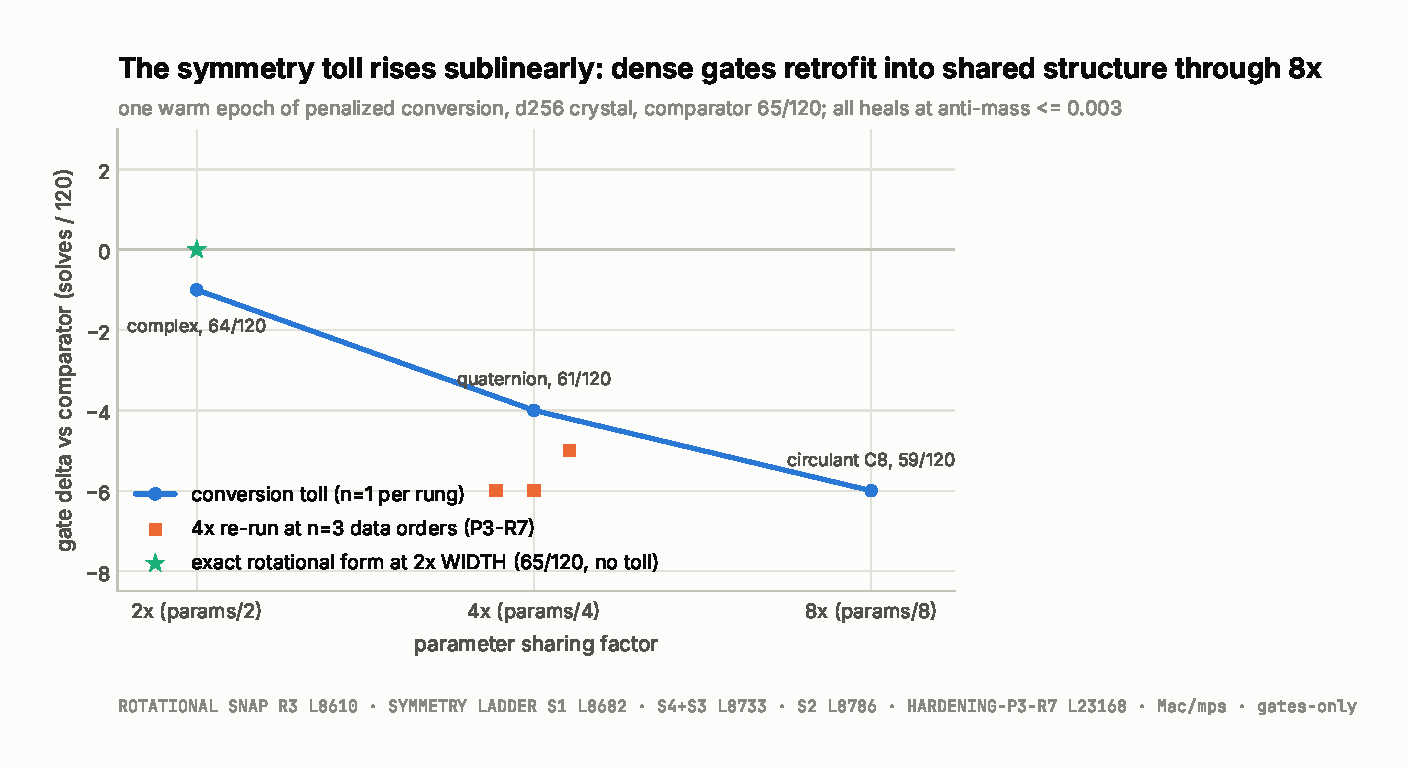
\includegraphics[width=0.86\linewidth]{symmetry_toll.pdf}
\caption{The symmetry toll curve (R3, S1, S3, S4, S2, and the P3-R7 hardening).
The claim: imposing a $k\times$ parameter-sharing group symmetry on a trained
crystal costs a small, roughly increasing number of solves, and an exact form
exists at $2\times$ width for the complex case.
% RESULTS L8616, L8690, L8742-8743, L8791, L23178
Fence: gates-only, MPS, $n{=}1$ per rung except the $4\times$ rung, which is
$n{=}3$ data-order seeds (pooled $-17$).}
\label{fig:toll}
\end{figure}

\paragraph{Discussion: the division-algebra reading is an analogy, not a
measurement.}
It is tempting to read Table~\ref{tab:ladder} as a Hurwitz ladder ---
$\mathbb{R}, \mathbb{C}, \mathbb{H}, \mathbb{O}$ at $1\times, 2\times, 4\times,
8\times$ --- with the toll as the price of losing commutativity and then
associativity. We label that framing explicitly as analogy, and we hold our own
counterexamples against it. The $8\times$ rung is \emph{not} octonions: it is
$C_8$ block-circulant structure, a cyclic-group convolution, which has nothing
to do with the octonion multiplication table. And $Z_2$ and complex sit at the
same $2\times$ sharing with different damage, which a division-algebra account
does not predict. The measured object is a toll curve in parameter sharing; the
algebraic story is decoration on top of it.

\section{The capacity meter as a predictive instrument}
\label{sec:capmeter}

The meter was pre-registered as a predicate before its read: at step
$\sigma_r/2$ per row, $M$ = span bits minus code-stream Shannon entropy,
param-weighted over 2-D weights, with three named predictions and a shipped
decision rule either way. % RESULTS L10783-10804
We record how it scored, because a meter's value is its calibration, not its
existence.

\begin{itemize}
\item \textbf{Prediction 1 (crystals in $1.5$--$2.5$): confirmed} --- crystals
read $0.96$--$1.61$, in band and if anything cleaner than predicted.
% RESULTS L10812-10819
\item \textbf{Prediction 2 (web-dense $\geq 4$): directional, not hit} ---
Qwen2.5-0.5B $3.62$ and SmolLM2-1.7B $3.85$. The separation from the crystal band
is clean, but the numeric threshold was missed by about $0.3$ and we book that
as a miss. % RESULTS L10820-10822
\item \textbf{Prediction 3 (MoE experts closer to crystals than to web-dense):
confirmed} --- DeepSeek-V3's routed experts read kurtosis 3.07 and $M\,2.33$.
% RESULTS L10822-10824
\end{itemize}

The instrument's real test came at C7, where it was used \emph{forward}. Packing
OLMoE's expert tensors at matched 6 bits, $\sigma$[row] read \dkl{} $0.0716$/tok
against rtn $0.0097$ and hqq $0.0044$ --- a $16.3\times$ premium to HQQ; the
dense attention control read $0.0442$ vs rtn $0.0053$ vs hqq $0.0020$, a
$22\times$ premium. % RESULTS L10897-10900
The strong-form transport prediction missed: OLMoE experts are not crystal-band
($M\,2.85$, kurtosis 3.50 --- Gaussian-shaped but wide-spanned).
% RESULTS L10901-10902
Crucially, the meter said so \emph{before} the arms ran: the kill-time amendment
recorded experts at $M\,2.85$, $0.35$ above the predicted band.
% RESULTS L10890-10893
That is the sense in which the premium is monotone in $M$ --- and the sense in
which kurtosis is demoted: 3.50 looked Gaussian, and span-priced $M$ caught what
the fourth moment missed. % RESULTS L10922-10924
The decision rule sharpened accordingly: $\sigma$-law only below $M \sim 2$.
% RESULTS L10916-10917
The wall-time prediction confirmed at scale: HQQ 675.5\,s on 6.4B expert
parameters against $\sigma$'s 16.6\,s, $41\times$. % RESULTS L10914-10915

The whole C-series was replicated on every arm: the C0/C1 rerun reproduced pack
stats and all four gates line-for-line; C4's cross-device integer invariance held
on a fresh activation battery; C6c's \dkl{} values reproduced to printed
precision; large-shape kernel speedups landed within 2\% of booked.
% RESULTS L10840-10850

\paragraph{Exploratory: an open lead at $M \approx 1.96$.}
A V4-Flash read puts a two-expert sample at $M \approx 1.96$. This is
\emph{exploration grade}: $n{=}2$ experts, no RESULTS booking, artifact rows in
\texttt{data/lake/weights.parquet} (L1E107, L29E13). We report it as an open lead
and draw no conclusion from it.

\section{Measured limits}
\label{sec:limits}

This section is not an appendix. The method has a boundary and we measured where
it is.

\paragraph{The falsifier fired on the first real LLM.}
Per-tensor $\sigma$ allocation does not transport to Qwen2.5-0.5B. Against an
fp16 control perplexity of 60.29, the $\sigma$ pack (avg raw 6.82 bits, matched
to 7) read \dkl{} $1.2839$/tok and ppl 96.39, against rtn7's $0.1669$/60.90 and
hqq7's $0.0388$/60.52. That is $33\times$ HQQ's \dkl{} --- the pre-registered
falsifier bar was $5\times$, and it fired decisively. Even plain RTN, with
per-row max scales, beats per-tensor $\sigma$ by $8\times$. % RESULTS L10678-10684

\paragraph{The granularity rescue failed.}
The obvious rescue --- keep the closed form but move to per-row grids --- did
not work: $\sigma$-pack[row] read \dkl{} $1.3072$/tok and ppl 90.26,
statistically unchanged from per-tensor. Prediction 1 falsified: no $\geq
10\times$ recovery. % RESULTS L10711-10714
Both arms anchor the step at $\sigma/2$, the crystal knee, and web-trained
Qwen's fragility constant is far larger than any crystal's.

\paragraph{The step rescue works, and still loses.}
Moving to step $\sigma/8$ ($q_r = \lceil 16/\sigma_r \rceil$, 9.64 raw bits
matched to 10) recovers $11.6\times$: \dkl{} $0.1127$/tok, ppl 60.64. The
$\sigma$ \emph{form} survives; the knee constant, not the allocation form, was
the failure. But rtn10 reads $0.0029$ and hqq10 $0.0007$ --- max-anchored grids
own heavy tails, and prediction 2 (within $2\times$ of rtn) was falsified.
% RESULTS L10738-10743
The mechanism is now clean: our fixed-width bits are priced by the worst
outlier's span, so one 50-sigma outlier inflates every row's bit count, while
max-anchored grids spend the same bits as a finer step on every quiet row.
% RESULTS L10744-10747
Among \emph{zero-calibration} methods, RTN is the one to beat, and on web-dense
weights we do not beat it; HQQ (0.0044) in turn beats RTN (0.0097) on the OLMoE
expert arm. % RESULTS L10898

\paragraph{Attacking the span is catastrophic.}
If outliers inflate the span, clip them. We pre-registered a $\sigma$-clip
allocator on SmolLM2-1.7B at 6 bits and it was destroyed: against an
rtn(absmax) baseline of \dkl{} 3.32 / ppl \textbf{62.98}, $k{=}4$ read \dkl{}
8.82 / ppl \textbf{138{,}890}; $k{=}6$ gave ppl 5{,}913; $k{=}8$ gave 532; hqq
read 0.445 / 61.96. % RESULTS L10949-10952
Saturating even the $>\!8\sigma$ tail kills the model. Web-dense outliers are
load-bearing at full magnitude, and the span attack is dead.

\paragraph{There is no universal distortion curve.}
Recomputing 21 historical snap cells onto a normalized distortion axis
$D/\sigma^2$, the cells are monotone \emph{within} each crystal but there is no
universal $f(x)$: at $x \approx 0.09$ the 19M crystal keeps 0.878 of its solves
while cplx\_none keeps 1.000; d56 bites by $x \approx 0.014$ where cplx is
untouched at $x \approx 0.12$ --- a $\sim$30$\times$ fragility spread at matched
normalized distortion. % RESULTS L10310-10315
The equation is two-parameter: kept $\approx f(k_c \cdot D/\sigma^2)$, with $f$
a universal monotone shape and $k_c$ a per-crystal fragility (rough fit:
cplx\_none 1, 19M $\sim$4--5, d56 $\sim$25--30). % RESULTS L10317-10319
Geometry-blindness survives this (polar and Cartesian cells interleave on the
same crystal's curve), but the knee \emph{constant} is crystal-priced --- and
$k_c$ is exactly what the entropy meter cannot see.

\begin{figure}[t]
\centering
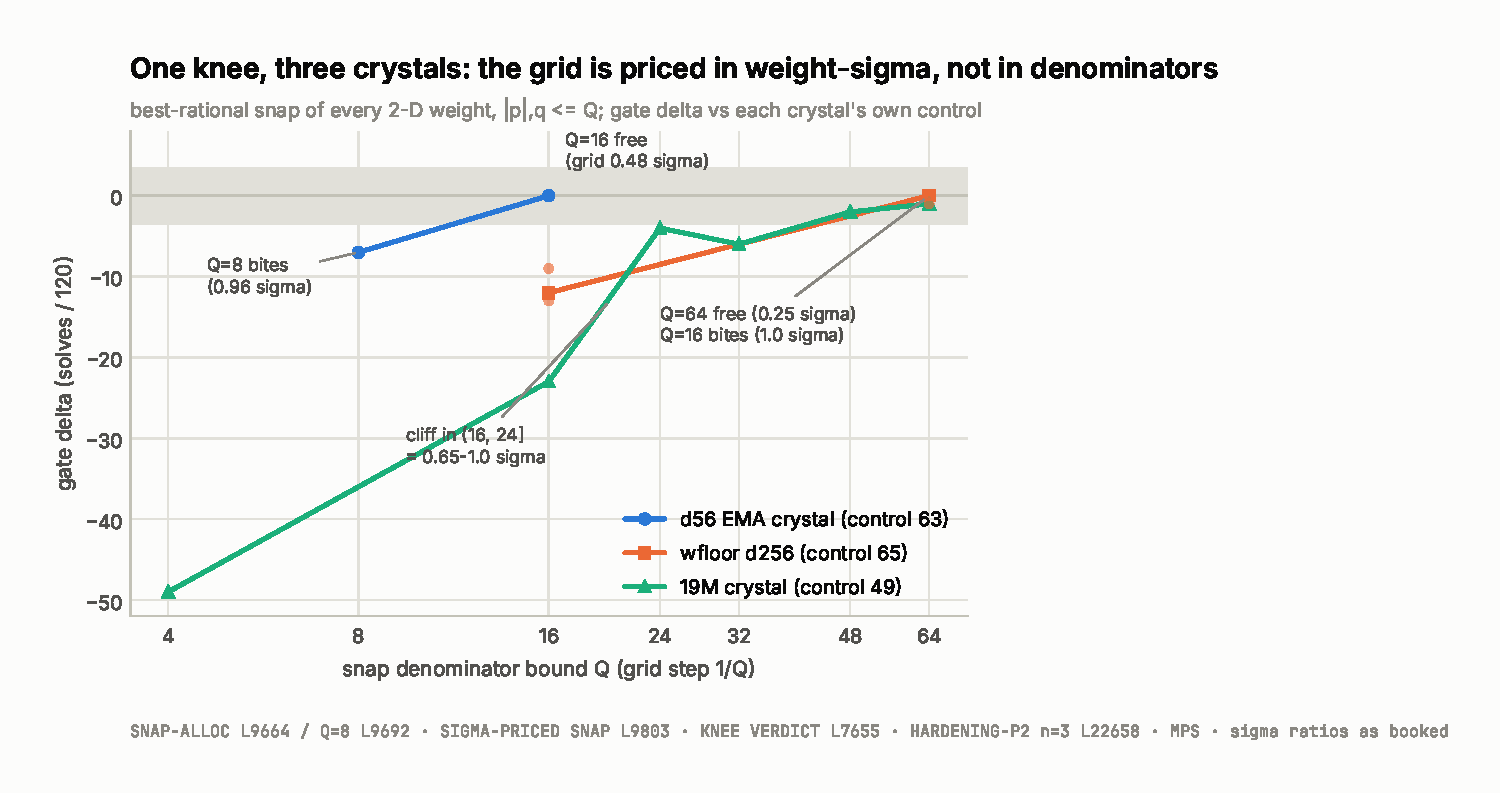
\includegraphics[width=0.86\linewidth]{quant_knee.pdf}
\caption{The precision knee in $\sigma$ units. The claim: the free/bites boundary
sits at a grid step of roughly $0.5$--$1.0\,\sigma$ regardless of width --- d56
$Q{=}16$ free (63/63/63 vs baseline 63) and $Q{=}8$ biting
($-4/-4/-7$); % RESULTS L9666, L9694
d256 $Q{=}64$ exactly free (65/65/65); % RESULTS L9805
19M sweep control 49 with $Q{=}16$ 26, $Q{=}24$ 45, $Q{=}32$ 43, $Q{=}48$ 47,
$Q{=}64$ 48. % RESULTS L7657-7658
Fence: the original cells are $n{=}1$, MPS, gates-only; the knee constant itself
is hardened to $n{=}3$ paired births ($Q{=}64$: $0/-1/0$; $Q{=}16$:
$-12/-13/-9$). % RESULTS L22662-22668
}
\label{fig:knee}
\end{figure}

\paragraph{The zero-tax claim's scope.}
Zero tax means: the d64h8 crystal class, at $n{=}3$, under \emph{outcome}
scoring, below $M \sim 2$. It does not extend to the L4 depth floor ($-5$ at two
seeds), % RESULTS L11239-11241
to per-token KL as the metric (rtn wins), % RESULTS L11137-11138
or to web-dense weights (Sec.~\ref{sec:limits}, first three paragraphs).

\paragraph{Fence inventory: what is $n{=}1$ and what is not.}
$n{=}3$: the C1 pack-parity headline on d64h8 and the entropy-bound gap;
% RESULTS L11234-11239
the precision knee constant; % RESULTS L22662
the quaternionic $4\times$ toll; % RESULTS L23178
the init-default causal leg for expert decorrelation. % RESULTS L22729-22735
$n{=}2$: the causal micro-MoE experiment (two seeds, house scale, one task
diet); % RESULTS L11630-11640
the cross-device integer hash (two activation batteries). % RESULTS L10842
$n{=}1$: every quantizer arm in C3; % RESULTS L10483
every meter row; every kernel shape; % RESULTS L10600
the C5 tier tax; the C6/C6b/C6c cells; the P2a-v2 clip arms;
% RESULTS L10693, L10945
each symmetry-ladder rung except the $4\times$; and both K3 cells.
% RESULTS L11459, L11524

\section{What routing does to weights}
\label{sec:routing}

The MoE rows of the dial ($M \sim 1.9$--$2.9$) invite an obvious post-hoc
program: find the redundancy between experts and compress it --- merge similar
experts, share bases, factor deltas. We measured the preconditions and closed the
program.

In weight space, production experts are decorrelated to numerical zero. On
Qwen3-30B, 128 gate\_proj experts decoded at layers 12 and 40 read
$\sigma(\text{delta})/\sigma(W) = 0.995 / 0.993$ with mean pairwise correlations
of $0.0024$ and $0.0054$ (max $0.0155$) --- there is no shared component for a
base-plus-delta factorization to extract. % RESULTS L11109-11115
This was a \emph{confirmed} house prediction, not a falsification: the pre-reg
predicted ratio $>0.8$ and correlations $\approx 0$, and both landed.
% RESULTS L11100-11112

But the redundancy did not vanish; it moved. Co-routing mutual information
between expert pairs \emph{within} a layer runs $0.21$--$0.46$ bits against a
token-shuffle scale of $0.0009$ --- roughly 300--500$\times$ baseline, at every
layer. % RESULTS L11168, L11193-11196
Merging the top-MI pair (layer 15, experts 1 and 29 --- the most co-routed pair,
not the most similar in weight space) costs perplexity $75.74 \to 79.10$, i.e.\
$+3.4$. % RESULTS L11169, L11197-11199
Storage-side redundancy became usage-side structure --- a systems lever
(prefetch, placement, caching, as the offloading literature already exploits),
not a parameters lever. % RESULTS L11201-11205

\paragraph{The causal experiment, and what it actually taught.}
We trained matched micro-MoEs (0.9M parameters, four experts, top-1 switch
routing, two seeds) under (a) the standard load-balance loss, (b) no balance
loss, and (c) tied base-plus-delta experts. Removing the balance loss changed
neither the decorrelation ($0.0080$ vs $0.0085$) nor the routing structure
($256\times$ vs $288\times$ shuffle), and the router did not collapse (worst
share 55\%). % RESULTS L11599-11608
Both readings replicated at seed 2 ($0.0082$ vs $0.0085$; MI $205\times$ vs
$299\times$). % RESULTS L11630-11636

Our first mechanism for this was that \emph{sparse assignment itself} creates the
split --- hard-routed experts never see the same tokens and so cannot stay
correlated. That mechanism is retracted. A soft-mixture arm, in which every
expert sees every token, landed correlation $0.0089$, indistinguishable from the
top-1 arms; the prediction of a $\geq 10\times$ rise under soft routing was
falsified, which kills the sparsity explanation. % RESULTS L11896-11903
The desk check that settles it: expert correlation \emph{at initialization} is
$0.0016$. % RESULTS L11904
Independently parameterized high-dimensional weight vectors start near-orthogonal
and training raises them only to $\approx 0.008$ in every regime tested; no
routing regime we ran supplies a force toward correlation. Decorrelation is the
\textbf{init default preserved}, not a product of routing. This causal leg is now
$n{=}3$ soft-routing seeds ($0.0096$, $0.0071$, $0.0062$, all far below the
$10\times$-over-$0.0016$ falsification criterion), on one device.
% RESULTS L22726-22739

Two riders. The production signature reproduces at 1/30{,}000th production scale
(corr $\approx 0.005$, MI 205--299$\times$ shuffle on a 0.9M-parameter
micro-MoE), making the phenomenon cheap to study. % RESULTS L11618-11620, L11640
And experts \emph{tied at birth} were booked as a \textbf{split} prediction, not
a clean win: the tied arm gates 43, the best MoE arm and within sigma of the
dense control at both seeds, so the tie pays almost nothing --- but the base does
\emph{not} dominate (deltas grew to $0.76$--$0.8\times$ base norm) and the deltas
stay $\sim7\times$ more correlated than untied experts. % RESULTS L11608-11612, L11637-11639
The factorization that post-hoc analysis proves impossible is approximately free
if imposed before training, and it does not compress the way the tie was supposed
to.

A seed-1 exploratory rider on $(M, \text{MI})$ opposite motion was killed
honestly: seed 2 showed no monotone relation and the MI ordering across arms
flipped ($205\times$ lb / $299\times$ free at seed 2, against $288\times$ /
$256\times$ at seed 1). % RESULTS L11616, L11630-11631, L11641-11642

\section{Related work}
\label{sec:related}

\paragraph{Calibrated PTQ.}
Our relationship to GPTQ \cite{gptq}, AWQ \cite{awq} and HQQ \cite{hqq} is not competitive but \emph{conditional}: on web-dense LLMs they earn
a $16$--$34\times$ premium over our closed form and we say use them; on
at-capacity networks they do not separate from it at gate resolution, and the
meter tells you which case you are in from the file alone, with no forward pass.
We are not aware of a prior pre-quantization regime test, though we make no claim
to have surveyed the space exhaustively.

\paragraph{Outlier methods.}
LLM.int8() \cite{llmint8} and SqueezeLLM \cite{squeezellm} rest on the premise
that outliers are load-bearing. Our clipping falsifier is direct evidence for
that premise from the opposite direction (clipping web-dense weights at
$4\sigma$ is catastrophic --- perplexity 138{,}890 against an rtn baseline of
62.98), % RESULTS L10949-10950
and $M$ is precisely a measure of the fixed-width price those outliers impose.

\paragraph{Information-theoretic codebooks.}
NF4's quantile codebooks \cite{qlora}, QuIP\#'s Hadamard incoherence processing
\cite{quipsharp}, AQLM's learned lattices \cite{aqlm} and TurboQuant's random
rotations \cite{turboquant} are a family of transforms \emph{toward} the Gaussian
regime. Our measurement is that convergent training on verified tasks produces
that regime natively, so we characterize the endpoint of the line the transforms
are walking.

\paragraph{Weight entropy coding.}
Deep Compression \cite{deepcompression} Huffman-codes pruned CNNs and DeepCABAC
\cite{deepcabac} arithmetic-codes them. Section~\ref{sec:rans} is the LLM-scale
revival, with the coding gain predicted in advance by the same statistic that
selects the quantization regime.

\paragraph{MoE structure.}
Switch \cite{switch} and DeepSeekMoE \cite{deepseekmoe} argue that fine-grained
experts specialize; Section~\ref{sec:routing} is the weight-space receipt. Expert
offloading systems \cite{moeoffload} implicitly bet on routing locality; our
co-routing MI is the statistic they are betting on, measured. REAP
\cite{reap} appears here as bibliographic context only: we did not run it, and
our merge probe is a single $n{=}1$ cell, so the most we can say is that our
result is not in tension with their report that merging carries irreducible
error versus pruning.

\paragraph{Determinism.}
Integer-only inference exists for edge CNNs \cite{jacob}. We are not aware of a
prior LLM decode with cross-vendor bit-identical logit traces, nor one executing
a frontier model's shipped format exactly; we state this as the limit of our
awareness rather than as a survey result.

\section{Fences}
\label{sec:fences}

Every scope limit, in one place.
\begin{enumerate}
\item The zero-tax parity claim is scoped to the d64h8 class at $n{=}3$
($+2/-3/0$, all sub-sigma against gate sigma 3.5; exact only at seed 1); the L4
depth floor pays $-5$ at both weak seeds. % RESULTS L11234-11241
Per-crystal fragility ($k_c$, near-tie flip density) is an orthogonal axis the
entropy meter does not see. % RESULTS L10317
\item The meter on quantized releases (Kimi-K2, Kimi-K3) reads the shipped grid's
image, not the fp master; the DeepSeek-V3 row is likewise a \emph{dequantized}
read (fp8 block-dequant, one shard). % RESULTS L10815, L11447
Those rows support bands, not rank orderings.
\item All paired comparisons are same-device, same-seed. The $2\times$
device-dependence figure belongs to the \emph{L9 probe} (the fp32 champion scored
18/24 on cuda vs 9/24 on MPS at the near-tie frontier); % RESULTS L3219-3220
at fp32 the production \emph{gate} measured a device delta of $-1$ (MPS 70 vs
cuda 69, sub-noise). % RESULTS L4737-4740
We do not compare gates across devices regardless.
\item The determinism claim is about the fixed-point path's own reproducibility;
it is not fp equivalence (96.66\% argmax agreement, disagreements at coin-flip
margins), and the reference implementation is 10--40$\times$ slower than fp.
% RESULTS L11370-11381
\item The cross-lab replication covers the Stage-2 (P3) fixed-point decode only.
The K3/MXFP4 cells are house-only across three backends; the second lab's leg was
MPS. % RESULTS L11479-11480, L11515
\item The Kimi-K3 cells are two experts metered and one hash-locked at GEMV and
full-chain level on a synthetic battery --- an expert \emph{forward}, not a
full-model decode. % RESULTS L11443, L11459, L11524
\item Wall-time wins in Sec.~\ref{sec:artifact} are calibration-time, not
inference-time, and both cells come from regimes where our quality claim failed;
where parity holds, calibration is sub-second. % RESULTS L10478-10481
\item Kernel speedups are $n{=}1$ per shape on synthetic Gaussian weights; the
headline is the best of five shapes and micro shapes are parity-within-noise.
% RESULTS L10600, L10850
\item Sections~\ref{sec:geometry} and \ref{sec:symmetry} are single-seed,
gates-only, MPS (ZX column: cuda), except the $4\times$ toll at $n{=}3$.
\item Cells at $n{=}1$ are named as such where they appear; see the fence
inventory in Sec.~\ref{sec:limits}.
\end{enumerate}

\section{Reproducibility}
\label{sec:repro}

Every experiment in this paper was pre-registered in an append-only log ---
predictions and falsifiers named before the run fired. Reads taken outside a
pre-registration are labelled exploratory in the log and in this text (the
$(M, \text{MI})$ rider and the V4-Flash lead are the two that appear here).
% RESULTS L11556, L11614
Every falsification appears in the text with the same prominence as the
confirmations; corrections are amendments naming their target, never edits. All
instruments, seeds, and the log itself are in the repository. Numeric artifacts
travel sha-pinned, and the replication protocol of Sec.~\ref{sec:determinism}
(pinned artifact, pinned instrument, full-digest compare) was validated by an
independent laboratory reproducing both hashes on first attempt.
% RESULTS L11471-11480

Where a result depends on a generated dataset, the generator uses stable string
seeds and exclusion-guarded train/eval splits. One contamination incident is
booked in the log itself: Holdout v1 was voided by its own audit at 281 corpus
collisions on the 88M band. % RESULTS L3276-3278
Two further incidents that motivated the same discipline (a mathgen L1/L2
eval-in-train overlap, and a generator whose \texttt{pick()} admitted only four
distinct bodies) are recorded in the repository's working-conventions file rather
than in the results log; we name the location so the count is not overstated.

\begin{thebibliography}{99}

\bibitem{gptq} E.~Frantar, S.~Ashkboos, T.~Hoefler, D.~Alistarh.
GPTQ: Accurate Post-Training Quantization for Generative Pre-trained
Transformers. arXiv:2210.17323.

\bibitem{awq} J.~Lin et al.
AWQ: Activation-aware Weight Quantization for LLM Compression and Acceleration.
arXiv:2306.00978.

\bibitem{hqq} H.~Badri, A.~Shaji.
Half-Quadratic Quantization of Large Machine Learning Models. Mobius Labs, 2023.
Software and blog release (no arXiv preprint).

\bibitem{llmint8} T.~Dettmers, M.~Lewis, Y.~Belkada, L.~Zettlemoyer.
LLM.int8(): 8-bit Matrix Multiplication for Transformers at Scale.
arXiv:2208.07339.

\bibitem{squeezellm} S.~Kim et al.
SqueezeLLM: Dense-and-Sparse Quantization. arXiv:2306.07629.

\bibitem{qlora} T.~Dettmers, A.~Pagnoni, A.~Holtzman, L.~Zettlemoyer.
QLoRA: Efficient Finetuning of Quantized LLMs. arXiv:2305.14314.

\bibitem{quipsharp} A.~Tseng et al.
QuIP\#: Even Better LLM Quantization with Hadamard Incoherence and Lattice
Codebooks. arXiv:2402.04396.

\bibitem{aqlm} V.~Egiazarian et al.
Extreme Compression of Large Language Models via Additive Quantization.
arXiv:2401.06118.

\bibitem{turboquant} TurboQuant: Online Vector Quantization with Near-Optimal
Distortion Error. arXiv:2504.19874 (ICLR 2026).

\bibitem{deepcompression} S.~Han, H.~Mao, W.~J.~Dally.
Deep Compression: Compressing Deep Neural Networks with Pruning, Trained
Quantization and Huffman Coding. arXiv:1510.00149.

\bibitem{deepcabac} S.~Wiedemann et al.
DeepCABAC: A Universal Compression Algorithm for Deep Neural Networks.
arXiv:1907.11900.

\bibitem{switch} W.~Fedus, B.~Zoph, N.~Shazeer.
Switch Transformers: Scaling to Trillion Parameter Models with Simple and
Efficient Sparsity. arXiv:2101.03961.

\bibitem{deepseekmoe} D.~Dai et al.
DeepSeekMoE: Towards Ultimate Expert Specialization in Mixture-of-Experts
Language Models. arXiv:2401.06066.

\bibitem{moeoffload} A.~Eliseev, D.~Mazur.
Fast Inference of Mixture-of-Experts Language Models with Offloading.
arXiv:2312.17238.

\bibitem{jacob} B.~Jacob et al.
Quantization and Training of Neural Networks for Efficient
Integer-Arithmetic-Only Inference. arXiv:1712.05877.

\bibitem{reap} M.~Lasby et al.
REAP: Router-weighted Expert Activation Pruning. arXiv:2510.13999 (ICLR 2026).

\end{thebibliography}

\end{document}
